\fig{fv:o3:matrix}{传播改变高度，薄透镜在同一高度改变光线倾角}{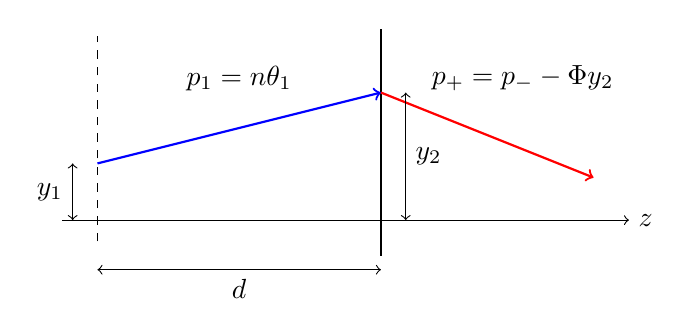
\begin{tikzpicture}[scale=.9]
\draw[->](-.5,0)--(7.5,0)node[right]{$z$};\draw[dashed](0,-.3)--(0,2.6);\draw[thick](4,-.5)--(4,2.7);
\draw[->,blue,thick](0,.8)--(4,1.8);\draw[->,red,thick](4,1.8)--(7,.6);
\draw[<->](0,-.7)--(4,-.7)node[midway,below]{$d$};
\draw[<->](-.35,0)--(-.35,.8)node[midway,left]{$y_1$};\draw[<->](4.35,0)--(4.35,1.8)node[midway,right]{$y_2$};
\node at(2,2){$p_1=n\theta_1$};\node at(6,2){$p_+=p_- -\Phi y_2$};
\end{tikzpicture}}
图\ref{fv:o3:matrix}把矩阵中的每一项落实到光线：均匀段有 $y_2-y_1=d\tan\theta_1\simeq dp_1/n$，倾角不变；薄透镜处高度连续，约化倾角突变 $-\Phi y_2$。所以从左向右追迹时，先作用的传播矩阵写在右边，后作用的透镜矩阵写在左边。若把次序颠倒，透镜使用的高度会由 $y_2$误变为 $y_1$，一般对应另一套装置。这个几何顺序是矩阵乘法次序的依据。
